\documentclass[12pt]{article}
\usepackage[charter]{mathdesign}
\usepackage[spanish]{babel}
\let\circledS\undefined % here - PS
\spanishdecimal{.}


\usepackage{cite}
\usepackage{fancyhdr}
\usepackage{multicol}
\usepackage[margin=2.4cm]{geometry}


%math packages
\usepackage{amsmath}
\usepackage{amssymb}
\usepackage{amsthm}
\usepackage{amsfonts}
\allowdisplaybreaks



%Figures dependences
\usepackage{pgf}
\usepackage{tikz}
\usepackage{float}
\usepackage{graphicx}
\usepackage{subcaption}
\usetikzlibrary{arrows}


%Text color box dependences
\usepackage{tcolorbox}
\usepackage{varwidth}
\tcbuselibrary{theorems}
\tcbuselibrary{breakable}
\tcbuselibrary{skins}


\setlength{\parskip}{2mm}
\setlength{\parindent}{0pt}

\renewcommand{\qedsymbol}{$\blacksquare$}
\addto\captionsspanish{\renewcommand{\proofname}{\textnormal{\textbf{Demostración}}}}
\DeclareSymbolFont{yhlargesymbols}{OMX}{yhex}{m}{n}
\DeclareMathAccent{\wideparen}{\mathord}{yhlargesymbols}{"F3}

%\renewcommand{\theenumi}{\alph{enumi}}

%Useful text commands
\newcommand{\ie}{\ensuremath{\text{i.e.}\ }}
\newcommand{\emphtext}[1]{\textbf{\emph{#1}}}


%Number sets
\newcommand{\N}{\ensuremath{\mathbb{N}}}
\newcommand{\Z}{\ensuremath{\mathbb{Z}}}
\newcommand{\Q}{\ensuremath{\mathbb{Q}}}
\newcommand{\R}{\ensuremath{\mathbb{R}}}
\newcommand{\C}{\ensuremath{\mathbb{C}}}

\newcommand{\positiveSet}[1]{\ensuremath{#1^+}}
\newcommand{\negativeSet}[1]{\ensuremath{#1^-}}
\newcommand{\nonnegativeSet}[1]{\ensuremath{#1^{\geq 0}}}

%Useful math commands
\newcommand{\ds}{\displaystyle}
\renewcommand{\max}[1]{\ensuremath{máx #1}}
\newcommand{\inverseOf}[1]{\frac{1}{#1}}
\newcommand{\fullMod}[2]{\equiv #1 \pmod{#2}}
\newcommand{\refTheorem}[1]{\textbf{Teorema #1}}
\newcommand{\refDefinition}[1]{\textbf{Definición #1}}
\newcommand{\inverseOfD}[1]{\ensuremath{\dfrac{1}{#1}}}

\newcommand{\showLine}{
    \setlength{\columnsep}{0.9cm}
    \setlength{\columnseprule}{0.2pt}
}
\newcommand{\hideLine}{
    \setlength{\columnsep}{0.4cm}
    \setlength{\columnseprule}{0pt}
}


% -- Geometry commads --
\renewcommand{\emptyset}{\varnothing}
\newcommand{\theTriangle}[1]{\ensuremath{\triangle #1}}
\newcommand{\homothety}[4]{\ensuremath{H\hspace{-1mm}\left(#1, #2\right) : #3 \to #4}}
\newcommand{\ratioCM}[6]{\ensuremath{\frac{#1 #4}{#4 #2} \cdot \frac{#2 #5}{#5 #3} \cdot \frac{#3 #6}{#6 #1}}}
\newcommand{\problemImage}[2]{
    \begin{center}
        \includegraphics[width=#2]{#1}
    \end{center}}

\newenvironment{solution}[1][]{
    \ifstrempty{#1}{
        \begin{proof}[\textnormal{\textbf{Solución}}]}
    {
        \begin{proof}[\textnormal{\textbf{Solución #1}}]}
    }{
    \end{proof}}
\theoremstyle{definition}

%With section
\newtheorem{section-lemma}{Lema}[section]
\newtheorem{section-example}{Ejemplo}[section]
\newtheorem{section-theorem}{Teorema}[section]
\newtheorem{section-problem}{Problema}[section]
\newtheorem{section-exercise}{Ejercicio}[section]
\newtheorem{section-corollary}{Corolario}[section]
\newtheorem{section-definition}{Definición}[section]

%Without section
\newtheorem{case}{Caso}
\newtheorem{example}{Ejemplo}
\newtheorem{problem}{Problema}
\newtheorem{remark}{Observación}
\newtheorem{corollary}{Corolario}

%Without numeration
\newtheorem*{note}{Nota}
\newtheorem*{definition}{Definición}


%Text Color Box styles
\newtcbtheorem[number within=section]{tcb-theorem-style}{Teorema}
{
    enhanced,
    frame empty,
    interior empty,
    coltitle = black,
    colbacktitle = gray!15!white,
    fonttitle = \bfseries,
    extras broken = {frame empty, interior empty},
    borderline = {0.3mm}{0mm}{black},
    breakable = true,
    top = 4mm,
    before skip = 3.5mm,
    attach boxed title to top left = {yshift = -3mm, xshift = 3mm},
    boxed title style = {boxrule = 0mm, borderline = {0.1mm}{0mm}{black}},
    varwidth boxed title,
    separator sign none, description delimiters parenthesis,
    description font=\bfseries,
    terminator sign={.\hspace{1mm}}
}
{theorem.tcb-label}

\newtcbtheorem[number within=section]{tcb-problem-style}{Problema}
{
    enhanced,
    frame empty,
    interior empty,
    coltitle = black,
    colbacktitle = white,
    fonttitle = \bfseries,
    extras broken = {frame empty, interior empty},
    borderline = {0.4mm}{0mm}{black},
    breakable = true,
    top = 4mm,
    before skip = 3.5mm,
    attach boxed title to top left = {yshift = -3mm, xshift = 3mm},
    boxed title style = {boxrule = 0.3mm, borderline = {0.3mm}{0mm}{black}},
    varwidth boxed title,
    terminator sign={.\hspace{1mm}}
}
{problem.tcb-label}

\newtcbtheorem[number within=section]{tcb-example-style}{Ejemplo}
{
    enhanced,
    frame empty,
    interior empty,
    coltitle = black,
    colback = white,
    colbacktitle = gray!15!white,
    fonttitle = \bfseries,
    borderline = {0.2mm}{0mm}{black},
    breakable = true,
    before skip = 3.5mm,
    after skip = 0mm,
    top = 1mm,
    bottom = 1mm,
    left = 1mm,
    right = 1mm,
    separator sign none, description delimiters parenthesis,
    description font=\bfseries,
    terminator sign={.\hspace{1mm}}
}
{example.tcb-label}

\newtcbtheorem[number within=section]{tcb-definition-style}{Definición}
{
    enhanced,
    frame empty,
    interior empty,
    coltitle = black,
    colbacktitle = gray!15!white,
    fonttitle = \bfseries,
    extras broken = {frame empty, interior empty},
    borderline = {0.3mm}{0mm}{black},
    breakable = true,
    top = 4mm,
    before skip = 3.5mm,
    attach boxed title to top left = {yshift = -3mm, xshift = 3mm},
    boxed title style = {boxrule = 0mm, borderline = {0.1mm}{0mm}{black}},
    varwidth boxed title,
    separator sign none, description delimiters parenthesis,
    description font=\bfseries,
    terminator sign={.\hspace{1mm}}
}
{definition.tcb-label}

\newtcbtheorem[number within=section]{tcb-lemma-style}{Lema}
{
    enhanced,
    frame empty,
    interior empty,
    coltitle = black,
    colbacktitle = white,
    fonttitle = \bfseries,
    extras broken = {frame empty, interior empty},
    borderline = {0.4mm}{0mm}{black},
    breakable = true,
    top = 4mm,
    before skip = 3.5mm,
    attach boxed title to top left = {yshift = -3mm, xshift = 3mm},
    boxed title style = {boxrule = 0.3mm, borderline = {0.3mm}{0mm}{black}},
    varwidth boxed title,
    separator sign none, description delimiters parenthesis,
    description font=\bfseries,
    terminator sign={.\hspace{1mm}}
}
{lemma.tcb-label}

\newtcolorbox[auto counter]{remark.tcb}[1][]
{
    breakable,
    title = Observación~\thetcbcounter.,
    colback = white,
    %colbacktitle = green!20!white,
    colbacktitle = gray!15!white,
    coltitle = black,
    fonttitle = \bfseries,
    bottomrule = 0pt,
    toprule = 0pt,
    leftrule = 2.5pt,
    rightrule = 0pt,
    titlerule = 0pt,
    arc = 2pt,
    outer arc = 2pt,
    colframe = black
}


%Enviroments section-x.tcb
\newenvironment{section-theorem.tcb}[1][]
{
    \ifstrempty{#1}
    {
        \begin{tcb-theorem-style}{}{}
    }
    {
        \begin{tcb-theorem-style}{#1}{}
    }
    }{
    \end{tcb-theorem-style}
}

\newenvironment{section-problem.tcb}
{
    \begin{tcb-problem-style}{}{}
    }{
    \end{tcb-problem-style}
}

\newenvironment{section-example.tcb}[1][]
{
    \ifstrempty{#1}
    {
        \begin{tcb-example-style}{}{}
    }
    {
        \begin{tcb-example-style}{#1}{}
    }
    }{
    \end{tcb-example-style}
}

\newenvironment{section-definition.tcb}[1][]
{
    \ifstrempty{#1}
    {
        \begin{tcb-definition-style}{}{}
    }
    {
        \begin{tcb-definition-style}{#1}{}
    }
    }{
    \end{tcb-definition-style}
}

\newenvironment{section-lemma.tcb}[1][]
{
    \ifstrempty{#1}
    {
        \begin{tcb-lemma-style}{}{}
    }
    {
        \begin{tcb-lemma-style}{#1}{}
    }
    }{
    \end{tcb-lemma-style}
}
\usepackage{float}

\title{Ecuaciones diofánticas lineales}
\author{Kenny J. Tinoco}
\date{Septiembre 2024}
\begin{document}

    \maketitle
    \section{Definiciones}

    Antes de empezar recordemos lo siguiente.

    \begin{definition.box}{Máximo divisor común}{}
        Dados $a,b \in \Z^{\neq 0}$, el máximo $d \in \positiveSet{\Z}$ tal que $d \mid a$ y $d \mid b$ es el máximo divisor común,
        y lo denotamos por $d = \mcd a b.$
    \end{definition.box}

    \begin{definition.box}{}{}
        Si $a,b \in \Z^{\neq 0}$ con $\mcd a b = 1$, entonces diremos que $a$ y $b$ son coprimos, primos relativos o primos entre sí.
    \end{definition.box}

    \begin{definition.box}{Combinación lineal}{}
        Dados los enteros $a_1, a_2, \ldots, a_k$ definimos una combinación lineal de los $a_i$ como un número de la forma
        \[
            a_1 x_1 + a_2 x_2 + \ldots + a_k x_k
        \]
        donde los $x_i$ son enteros cualesquiera.
    \end{definition.box}

    \begin{theorem.box}{Algoritmo de la división}{}
        Si $a, b \in \Z$ con $b \neq 0$, entonces existen enteros únicos $(q,r)$ tales que $a = bq + r$ con $0 \leq r < |b|$.
    \end{theorem.box}

    Con el siguiente resultado es un teorema muy conocido e importante en la teoría de números y con el damos inicio al
    estudio de las ecuaciones diofánticas lineales, este resultado es utilizado tanto para la demostración de teoremas como
    la resolución de problemas.
    \begin{theorem.box}{Bezout}{}
        Si $d = \mcd a b$, entonces $d$ es el menor entero tal que
        \[
            ax + by = d,\ \text{para enteros}\ x,y.
        \]
    \end{theorem.box}
    \begin{proof}
        Sea $S$ el conjunto de todos los enteros $k$ tales que $ax + by = k$, debido a que la ecuación es sobre los números
        enteros podemos asegurar que $S$ no es vacío, por lo tanto, debe existir un elemento mínimo $k_1$.
        Con esto, nuestro objetivo será demostrar que $k_1 = \mcd a b$.
        Sin embargo, como $k_1$ es una combinación lineal de $a,b$ esto implica que $k_1$ es múltiplo de $\mcd a b$,
        con lo cual solo basta probar que $k_1 \mid a$ y $k_1 \mid b$, pero si esto es así, es equivalente a probar que
        $k_1$ divide a cualquier combinación lineal de $a,b$, es decir, todo elemento de $S$.
        Procedamos por contradicción, sea $n \in S$ un elemento cualquiera y digamos que $k_1$ no divide a $n$, por el
        algoritmo de la división tenemos que $n = k_1 q + r$ para algunos enteros $q, r$ con $0 < r < k_1$.
        Ahora bien, como $n$ y $k_1$ son combinaciones lineales de $a,b$, entonces $r = n - k_1 q$ también es combinación lineal.
        Por lo tanto, $r$ es un entero positivo menor a $k_1$ que pertenece a $S$, lo cual es una contradicción a la minimalidad de $k_1$.
        Luego, $k_1$ divide a todo $n \in S$ y por consiguiente $k_1 = \mcd a b$.
    \end{proof}

    \begin{theorem.box}{}{theorema3}
        La ecuación diofántica $ax + by = c$ tendrá soluciones si y solo si $\mcd a b \mid c$.
        Además, si $(x_0,y_0)$ es una solución particular, entonces la solución general es
        \[
            (x,y) = \left(x_0+\frac{b}{d}t,\ y_0 -\frac{a}{d}t\right) \quad \text{con}\ t \in \Z.
        \]
    \end{theorem.box}

    \begin{proof}
        Veamos la primera premisa, si $d = \mcd a b$, entonces $a = a_1 d$ y $b = b_1 d$, sustituyendo en la ecuación original
        obtenemos que $d (a_1 x + b_1 y) = c$ por lo cual $d$ divide a $c$.
        Ahora, por el teorema de bezout existen $x_1, y_1$ tales que
        \[
            ax_1 + by_1 = d.
        \]
        Ya que $c = kd$, al multiplicar el resultado anterior por $k$, obtenemos
        \[
            a k x_1 + b k y_1 = kd \iff a (kx_1) + b (ky_1) = c,
        \]
        donde las soluciones son $(x,y) = (kx_1, ky_1)$.
        Veamos la segunda premisa, sea $(x_0, y_0)$ una solución de la ecuación, al sustituir en la ecuación original, vemos que
        \begin{align*}
            ax + by &= c = ax_0 + by_0 \\
            \iff a(x - x_0) &= b (y_0 - y) \\
            \iff a_1 d(x - x_0) &= b_1 d (y_0 - y) \\
            \iff a_1 (x - x_0) &= b_1 (y_0 - y)
        \end{align*}
        Como $a_1$ y $b_1$ son coprimos, tenemos que $b_1 \mid (x - x_0)$ por lo cual $(x - x_0) = b_1 t$ donde $t$ es entero,
        sustituyendo en el resultado anterior, obtenemos $(y_0 - y) = a_1 t$, luego las soluciones son
        \[
            (x,y) = (x_0 + b_1 t, y_0 - a_1 t),\quad\text{con}\ a_1 = \frac{a}{d}, \ b_1 = \frac{b}{d}.\qedhere
        \]
    \end{proof}

    Ahora veamos algunos ejemplos.

    \begin{example}
        Resolver la ecuación $5x - 3y = 52$ en enteros positivos.
    \end{example}
    \begin{solution}
        Primero, como $\mcd 5 3 = 1$ y $1 \mid 52$, entonces la ecuación tiene soluciones enteras.
        Ahora, analizando en módulo 5 tenemos que
        \[
            - 3y \modulo{52}{5} \implies 2y \modulo{2}{5} \implies y \modulo{1}{5}.
        \]
        Claramente $y = 1$ es solución a esta congruencia, sustituyendo en la ecuación original $5x - 3\cdot 1 = 52 \iff 5x = 55$
        por lo cual, la ecuación tiene una solución $(11, 1)$, luego con la solución $(x_0,y_0)=(11,1)$ llegamos a
        \[
            (x,y) = (11+3t,1-5t),\ \text{donde}\ t\in \Z.\qedhere
        \]
    \end{solution}

    \begin{example}
        Resolver la siguiente ecuación $8c+7p=100$.
    \end{example}
    \begin{solution}
        Claramente la ecuación tiene soluciones enteras, analizando en módulo 8,
        \[
            7p \modulo{100}{8} \implies -p \modulo{4}{8} \implies p \modulo{-4}{8} \implies p \modulo{4}{8}.
        \]
        Rápidamente, podemos decir que $p = 4$ es una solución para dicha congruencia, sustituyendo en la ecuación obtenemos $c = 9$.
        Luego, con la solución $(c_0, p_0) = (9, 4)$ tenemos
        \[
            (c,p) = (9 + 7t, 4 - 8t),\quad \text{con}\ t\in \Z.\qedhere
        \]
    \end{solution}



    \section{Aplicando el algoritmo de Euclides}

    \begin{definition.box}{Algoritmo de Euclides}{}
        Si $a, b \in \Z^{\neq 0}$ y $a = bq + r$ para algunos enteros $q,r$ con $0 < r < b$, entonces
        \[
            \mcd a b = \mcd b r.
        \]
    \end{definition.box}

    Podemos usar este algoritmo para resolver ecuaciones lineales de una manera iterativa, similar, a la manera en cómo
    se calcula el MCD de dos números grandes.

    Sean $a,b, c \in \Z$ con $a,b \neq 0$ y $d = \mcd a b$, considerando la ecuación
    \[
        ax + by = c,
    \]
    se tienen los siguientes pasos:
    \begin{enumerate}
        \item Si $d\nmid c$, entonces no hay solución.
        \item Si $d \mid c$, entonces se divide la ecuación por $d$ obteniendo $a_1 x + b_1 y = c_1$.
        \item Por el paso anterior la ecuación tiene coeficiente coprimos;
        \begin{enumerate}
            \item[3.1.] Si $a_1 \mid c_1$, entonces $a_1 c_0 = c_1$, luego $(x,y) = (c_0, 0)$ es solución.
            \item[3.2.] Si $a_1 \nmid c_1$, entonces tomamos el menor de $|a_1|, |b_1|$ y obtenemos\footnote{Aquí vamos suponer que $|a_1|$ es el menor.}
            \begin{align*}
                b_1 = a_1 q_1 + r_1,\ \text{con}\ 0<r_1<|a|, && c_1 = a_1 q_2 + r_2,\ \text{con}\ 0 < r_2 < |a|.
            \end{align*}
        \end{enumerate}
        \item Sustituimos en la ecuación
        \[
            a_1 x + (a_1 q_1 + r_1) y = a_1 q_2 + r_2 \iff a_1 (x + q_1 y - q_2) + r_1 y = r_2.
        \]
        Haciendo $z = x + q_1 y - q_2$, la ecuación anterior se transforma en $a_1 z + r_1 y = r_2$.
        \begin{enumerate}
            \item[4.1.] Si $r_1 \mid r_2$, entonces terminamos con el paso 3.1.
            \item[4.2.] Si $r_1 \nmid r_2$, entonces vamos al paso 3.2 y repetimos el proceso.
        \end{enumerate}
    \end{enumerate}

    Con estos pasos (o algoritmo) es posible resolver ecuaciones diofánticas lineales con coeficientes grandes, de una manera
    cíclica o iterativa, lo cual reduce la complejidad de resolver la ecuación diofántica, esto lo podemos apreciar en la
    figura 1.
    \begin{figure}[H]
        \centering
        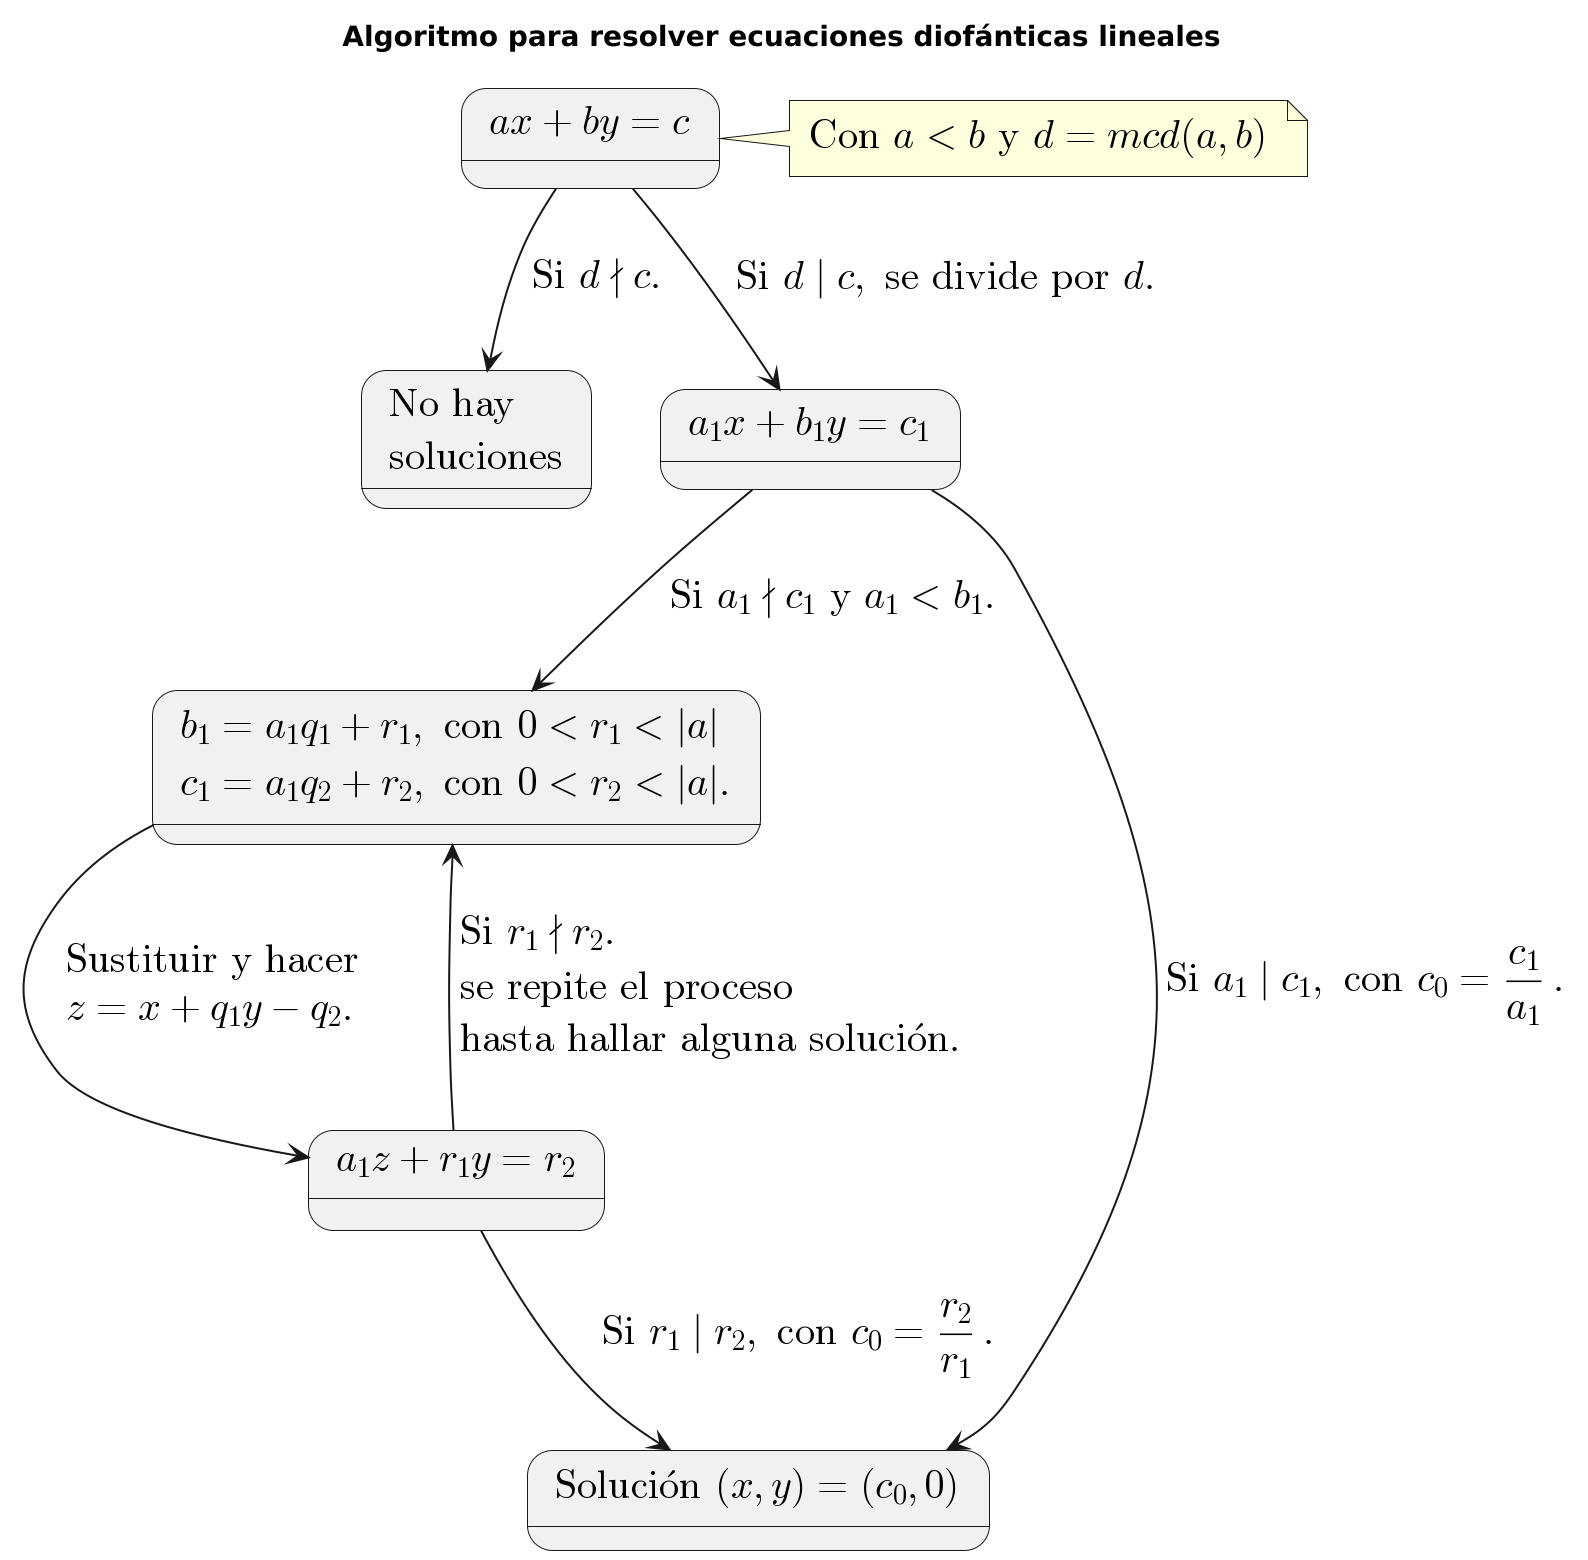
\includegraphics[width=\textwidth]{aplicando-algoritmo-de-euclides}
        \caption{Diagrama de estado para resolver ecuaciones diofánticas lineales.}
    \end{figure}

    Veamos algunos ejemplos.

    \begin{example}
        Resuelva la siguiente ecuación $350x + 425y = 1200$.
    \end{example}
    \begin{solution}
        Como $\mcd{350}{425} = 25$ y $25 \mid 1200$, dividimos ambos lados de la ecuación por $25$ y tenemos
        \[
            14x+17y=48
        \]
        Por el algoritmo de euclides se tiene que $17 = 1\cdot14+3$ y $48=3\cdot14+6$.
        Sustituyendo y agrupando, tenemos $14(x+y-3)+3y=6.$
        Haciendo $z=x+y-3$ y sustituyendo en esta última ecuación se tiene $14z+3y=6.$
        Como $3\mid6$, para esta ecuación tenemos una solución de la forma $z=0$ y $y=2$.
        Escribiendo $z$ en términos de $x$ y $y=2$, obtenemos el valor de $x=1$.
        Luego, la solución general de la ecuación inicial es:
        \[
            x=1+17k, \quad y=2-14k, \quad\text{con}\ k \in \Z. \qedhere
        \]
    \end{solution}



    \section{Caso general de ecuaciones lineales}

    Hasta el momento sólo hemos trabajado en ecuaciones lineales de dos variables, pero en realidad la ecuación $ax+by=c$ no es más que un caso particular de la ecuación
    \[
        a_1 x_1 + a_2 x_2 + \ldots + a_n x_n = c,
    \]
    donde $a_1, a_2, \dots, a_n,$ y $c$ son coeficientes.
    También, cabe mencionar que el teorema de bezout también se cumple para una cantidad $n$ de números, con lo cual
    se podrá hacer un tratamiento similar al caso concreto de $n = 2$.

    \begin{theorem.box}{}{}
        La ecuación diofántica $a_1 x_1 + a_2 x_2 + \ldots + a_n x_n = c$ tiene solución si y solo si $\mcd {a_1}{a_2,\cdots,a_n} \mid c.$
    \end{theorem.box}

    Veamos un ejemplo.

    \begin{example}
        Resuelva la ecuación $3x + 4y + 5z = 6$.
    \end{example}
    \begin{solution}
        Primero, notamos que $\mcd{3}{4,5} = 1$ efectivamente divide a 6.
        Trabajando en módulo 5 tenemos que $3x + 4y\modulo{1}{5}$ por lo cual $3x + 4y = 1 + 5s$, con $s \in \Z$.
        Si tomamos a $s$ como una constante, una solución para esta ecuación es $(x_0, y_0) = (-1 + 3s, 1 - s)$.
        Usando el teorema~\ref{t:theorema3}, obtenemos las soluciones generales de esta ecuación de dos variables
        \[
            (x,y) = (-1+3s+4t, 1-s-3t)\quad\text{con}\ t \in \Z.
        \]
        Sustituyendo esto en la ecuación original obtenemos $z = 1 - s$, por lo que todas las soluciones son
        \[
            (x,y,z)=(-1+3s+4t,1-s-3t,1-s), \quad \text{con}\ s,t \in \Z.\qedhere
        \]
    \end{solution}

    Como vemos en este ejemplo, una ecuación de tres variables la podemos reducir a una ecuación de dos variables,
    ecuación que sabemos cómo solucionarla, luego solo debemos revertir el proceso y dejar las soluciones en función
    de los parámetros que aparezcan.
    Análogamente, podemos resolver una ecuación de grado $n$ reduciéndola sucesivamente a una de grado dos y realizar un proceso similar.


    \section{Existencia de soluciones}

    Para concluir, veremos algunos resultados que estudian la existencia de soluciones para una ecuación diofántica, estos
    resultados ya son parte de una teoría de mayor complejidad, si se tiene curiosidad se invita al lector a investigar más a fondo.

    \begin{definition.box}{}{}
        Sean  $a_1,a_2,\ldots,a_n$ enteros positivos con $\mcd{a_1}{a_2,\ldots,a_n} = 1$ se define a $g(a_1,a_2,\ldots,a_n)$
        como el mayor entero positivo $N$ para el cual
        \[
            a_1 x_1 + a_2 x_2 + \ldots + a_n x_n = N,
        \]
        no tiene soluciones enteras.
    \end{definition.box}

    El problema de determinar $g(a_1,\ldots,a_n)$ es conocido como el problema de las monedas de Frobenius.
    Este problema fue planteado por Ferdinand Frobenius, quien se interesó en encontrar la mayor cantidad de dinero que no
    se puede representar como una combinación lineal de $n$ denominaciones de monedas,
    quizás el ejemplo más sencillo es con monedas de 3 y 5 centavos con las cuales nunca se podrá pagar una deuda de 7 centavos.
    El siguiente teorema brinda un valor de $N$ para el caso de $n=2$.

    \begin{theorem.box}{Sylvester}{}
        Sean $a,b \in \positiveSet{\Z}$, con $\mcd a b = 1$, entonces
        \[
            g(a,b) = ab - a - b.
        \]
    \end{theorem.box}
    Con esto se puede analizar la ecuación $3x + 5y = 7$, como $g(3,5) = 3\cdot 5 - 3 - 5 = 7$
    entonces se tiene que 7 es el mayor entero para el cual no hay soluciones.
    Para los casos de $n\geq2$ hasta la fecha no se conoce ninguna fórmula explícita de $g$, cabe aclarar que estos temas
    ya son de una complejidad mayor a este curso.
    Finalmente, con el teorema sylvester podemos entender mejor el siguiente resultado.

    \begin{theorem.box}{Chicken McNugget}{}
    Sean\footnote{Su historia es curiosa, debido a que fue enunciado en un McDonald's.} $a, b\in \positiveSet{\Z}$ con $\mcd a b = 1$, se tiene:
    \begin{enumerate}
        \item[i.] Si $n = ab - a - b$, entonces $ax + by = n$ es insoluble $\forall x, y \in \positiveSet{\Z}$.
        \item[ii.] Si $n > ab - a - b$, entonces la ecuación es soluble.
    \end{enumerate}
    \end{theorem.box}
    Como recomendación general, se aconseja siempre verificar que una ecuación cumpla con el segundo punto del teorema anterior.




    \section{Ejercicios y problemas}

    Ejercicios y problemas para el autoestudio.

    \begin{exercise}
        ¿Tiene la ecuación $24x + 18y = 12$ soluciones enteras?
    \end{exercise}

    \begin{exercise}
        Resuelva la ecuación diofántica $125x - 25y = 28.$
    \end{exercise}

    \begin{exercise}
        Resuelva la ecuación $69x + 123y = 3000.$
    \end{exercise}
\end{document}